\documentclass[12pt,a4paper]{article}
\usepackage[utf8]{inputenc}
%\usepackage[spanish]{babel}
\usepackage{amsmath}
\usepackage{amsfonts}
\usepackage{amssymb}
\usepackage{graphicx}
\newcommand*{\qed}{\hfill\ensuremath{\blacksquare}}
\setlength{\parindent}{0pt}
\pretolerance=2000
\tolerance=3000
\author{Santiago de Diego, Jesús Bueno, Fernando de la Cruz, Javier Ruiz}
\title{Cadenas de Markov en tiempo continuo}
\date{}
\begin{document}
\maketitle
\newtheorem{theorem}{Teorema}[section]
\newtheorem{lemma}{Lema}[section]
\newtheorem{proof}{Demostración}[section]
\newpage
\tableofcontents
\newpage
\section{Introducción}
\subsection{Cadenas de Markov}
Primero de todo, presentamos una introducción a las Cadenas de Markov de forma genérica. Como ya sabemos, las cadenas de Markov son procesos de corta memoria en el sentido de que solo recuerdan el último estado visitado para decidir cual sería el próximo. En procesos con larga memoria el valor que toma el proceso en cada paso depende de todo el pasado.

Formalizando el concepto, el proceso $\{\mathbb{X}_n \}_{n\in \mathbb{N}}$ con espacio de estados $E$ es una cadena de Markov si:

$$P(\mathbb{X}_{n+1}=y \, | \, \mathbb{X}_n = x_n , \ldots , \mathbb{X}_0 = x_0)=P(\mathbb{X}_{n+1}=y \, | \, {\mathbb{X}_n=x_n})$$

Este tipo de procesos estocásticos tienen mucho interés a la hora de modelar determinados fenómenos, como por ejemplo el tiempo de espera a un servidor en función de la tasa de llegada de los clientes.

\subsection{Diferencia entre tiempo discreto y tiempo continuo}
La principal diferencia entre cadenas de Markov en tiempo discreto y tiempo continuo es, como dice el propio nombre, el tiempo. En las cadenas de Markov en tiempo continuo, consideramos un $t\in T \subset \mathbb{R}$ mientras que en las cadenas de Markov en tiempo discreto, trabajamos con instantes de tiempo de la forma $t\in \mathbb{N}$.
\section{Definición y propiedades}
\subsection{Definición}
Primero de todo, definiremos una Cadena de Markov como:
\\\\
\textbf{Definición: Cadena de Markov}
\\
Sea $\{\mathbb{X}_t\}_{t\geq 0}$ un proceso estocástico en tiempo continuo, esto es, $t\in [0,T]$ con $T\in \mathbb{R}$ que toma valores en un conjunto numerable $E$. Decimos que $\{\mathbb{X}_t\}_{t\geq 0}$ es una Cadena de Markov en tiempo continuo si $\forall t,s\geq 0$ y $\forall i,j,x_u\in E$ con $0\geq u \geq s$, se cumple que:
$$P(\mathbb{X}_{t+s}=j \, | \, \mathbb{X}_s =i \, , \,  \mathbb{X}_u =  u \,\, \forall 0\leq u\leq s)=P(\mathbb{X}_{t+s}=j \, | \, \mathbb{X}_s = i)$$
Es decir, podemos definir una Cadena de Markov como un proceso estocástico	en el que el futuro sólo depende del presente, independientemente de sus estados pasados. Además también podemos considerar la definición alternativa:
\\\\
\textbf{Definición 2: Cadena de Markov}
\\
El proceso estocástico $\{\mathbb{X}_t \, , \, t\in [0,\infty]\}$ es una Cadena de Markov en tiempo continuo si para cualquier entero $n\geq 0$, cualesquiera $0\leq t_0 < t_1 < \ldots < t_{n+1}$ y $i_0,\ldots , i_n,i_{n+1}\in S$ se verifica:
$$P(\mathbb{X}_{t_{n+1}}=i_{n+1}\, | \, \mathbb{X}_{t_0}=i_0 , \ldots \mathbb{X}_{t_n}=i_n)=P(\mathbb{X}_{t_{n+1}}=i_{n+1}\, | \, \mathbb{X}_{t_n}=i_n)$$\\
Además, introducimos también el concepto de Cadena de Markov en tiempo continuo homogénea:
\\\\
\textbf{Definición: Cadena de Markov homogénea en tiempo continuo}
\\
Una CMTC se dice homogénea si la probabilidad de ir del estado $i$ al estado $j$ no depende del instante de tiempo en el que se encuentra la cadena, formalmente esto es:
$$P(\mathbb{X}_n=j \, | \, \mathbb{X}_{n-1}=i)=P(\mathbb{X}_1=j \, | \, \mathbb{X}_0=i)$$
Una vez vistas estas definiciones podemos ver las propiedades de una Cadena de Markov.
\subsection{Propiedades}
Podemos notar dos propiedades fundamentales en cuanto a CMTC, que son:
\subsubsection{Primera propiedad}
$P(\mathbb{X}_{t_{n+h}}=i_{n+h}, h=1,\ldots m \, | \, \mathbb{X}_{t_k}=i_k, k=0,\ldots ,n)=P(\mathbb{X}_{t_{n+h}}=i_{n+h}, h=1,\ldots m\, |\, \mathbb{X}_{t_n}=i_n )$
\\
$\forall 0 \leq t_1< t_2, \ldots , < t_n+m\, , \forall i_k\in S, k=0,\ldots , n+m$
\begin{proof}
Vamos a demostrarlo por inducción:
\\\\
Primero hacemos el caso $h=1$:
\\\\
$P(\mathbb{X}_{t_{n+1}}=i_{n+1},h=1 \, |\, \mathbb{X}_{t_k}=i_k\, k=0,\ldots n)=P(\mathbb{X}_{t_{n+1}}=i_{n+1}\, | \,\mathbb{X}_{t_n}=i_n)$
\\
$\forall 0\leq t_1<t_2<\ldots <t_{n+m}\, \forall m\geq 1$ y $\forall i_k \in S, \,k=0,\ldots n+m$
\\\\
Lo suponemos cierto para $h$ y lo probamos para $h+1$:
\\\\
$P(\mathbb{X}_{t_{n+h}}=i_{n+h},\, h=1,\ldots m \, | \, \mathbb{X}_{t_k}=i_k ,\, k=0,\ldots n)P(\mathbb{X}_{t_k}=i_k,\, k=0\ldots n)$
\\
$=P(\mathbb{X}_{t_k}=i_k\, k=0,\ldots ,n+m+1)=P(\mathbb{X}_{t_{n+m-1}}=i_{n+m-1}\, | \, \mathbb{X}_{t_k}=i_k,\, k=0,\ldots , n+m)=P(\mathbb{X}_{t_k}=i_k,\, k=0,\ldots n+m)=P(\mathbb{X}_{t_{n+m+1}}=i_{n+m+1}\, | \, \mathbb{X}_{t_k}=i_k,\, k=0,\ldots ,n+m)=P(\mathbb{X}_{t_{n+h}}=i_{n+h},\, h=1,\ldots m \, | \, \mathbb{X}_{t_k}=i_k ,\, k=0,\ldots n)P(\mathbb{X}_{t_k}=i_k,\, k=0\ldots n)$
\\
$=P(\mathbb{X}_{t_{n+m+1}}=i_{n+m+1}\, | \, \mathbb{X}_{t_k}=i_k,\, k=0,\ldots ,n+m)P(\mathbb{X}_{t_{n+h}}=i_{n+h},\, h=2,\ldots m \, | \, \mathbb{X}_{t_k}=i_k ,\, k=0,\ldots n)P(\mathbb{X}_{t_k}=i_k,\, k=0\ldots n)$
\\\\
Obtenemos que:
\\\\
$P(\mathbb{X}_{t_{n+h}}=i_{n+h},\, h=1,\ldots m+1 \, | \, \mathbb{X}_{t_k}=i_k ,\, k=0,\ldots n)=P(\mathbb{X}_{t_{n+m+1}}=i_{n+m+1})P(\mathbb{X}_{t_{n+h}}=i_{n+h},\, h=1,\ldots m\, | \, \mathbb{X}_{t_n}=i_n)$
\\\\
Sin más que aplicar la definición tenemos que lo anterior es igual a $P(\mathbb{X}_{t_{n+m+1}}\, | \, \mathbb{X}_{t_n}=i_{t_n})$
\qed
\end{proof}
\subsubsection{Segunda propiedad}
\begin{proof}

\end{proof}
\subsection{Relación con la teoría de autómatas}
En concreto, podemos asociar a una cadena de Markov un grafo, como veremos más abajo. De esta forma, el grafo resultante se comporta de igual manera que un \textbf{autómata finito determinista}, relacionándose de esta forma las cadenas de Markov con la teoría de autómatas.
\\\\
Primero de todo, vamos a definir el grafo de una CMTC ya que resulta fundamental para entender lo siguiente:
\\\\
\textbf{Definición: Grafo asociado a una CMTC}
\\
$G=(E,U,W)$ es el grafo asociado a una CMTC sii:
\begin{itemize}
\item $E$ es el conjunto de estados de la cadena
\item $U$ es el conjunto de aristas, que en este caso sería el conjunto de transiciones posibles
\item $W$ es el conjunto de ponderaciones. Podemos verlo como el conjunto de valores de cada arista
\end{itemize}
Además $G$ es un grafo orientado, es decir, que tenemos en cuenta cual es el nodo origen y cual es el nodo destino.
\\\\
Una vez presentada la definición de grafo asociado a una CMTC, podemos establecer una biyección entre el conjunto de grafos orientados asociados a una CMTC y el conjunto de los autómatas finitos deterministas, aunque estos resultados se escapan del alcance del trabajo en cuestión. Simplemente mostraremos un ejemplo de uno de estos grafos:
\\
\begin{figure}[h]
  \centering
    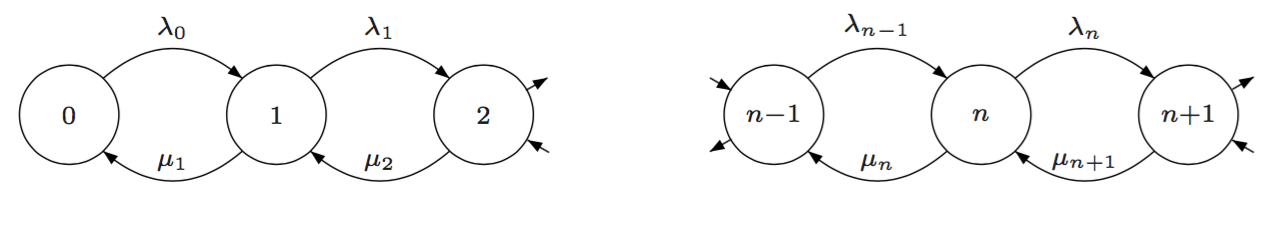
\includegraphics[width=0.7\textwidth]{img/grafo.png}
  \caption{Ejemplo de grafo de una CMTC-h}
  \label{fig:ejemplo}
\end{figure}
\\
En el grafo de la izquierda aparecen 3 estados, que corresponden a las variables aleatorias $\mathbb{X}_{t_1}$, $\mathbb{X}_{t_2}$ y $\mathbb{X}_{t_3}$ y representadas como $\lambda_0$, $\lambda_1$, $\mu_1$, $\mu_2$ aparecen las 4 probabilidades de transición. Por último, las flechas indican la dirección en la que se produce la transición.
\\\\
El grafo de la derecha es idéntico pero corresponde a las variables aleatorias $\mathbb{X}_{t_{n-1}}$, $\mathbb{X}_{t_n}$ y $\mathbb{X}_{t_{n+1}}$. Además, según lo visto anteriormente tenemos que el grafo corresponde a la manera usual de representar un autómata finito determinista.
\\\\
Para concluir presentaremos la definición de autómata finito determinista, por si el lector está interesado en el estudio del mismo:
\\\\
\textbf{Definición de autómata finito determinista:}
\\
Un AFD es una 5-tupla $(Q,\sum ,q_0,\delta,F)$ donde:
\begin{itemize}
\item $Q$ es un conjunto de estados
\item $\sum$ es un alfabeto
\item $q_0$ es el estado inicial
\item $\delta :Q\times\sum\rightarrow Q$ es la función de transición
\item $F\subseteq Q$ es el conjunto de estados finales
\end{itemize}
Además verifica que $\delta (q,a)=q_1$ y $\delta (q,a)=q_2 \Rightarrow q_1 \neq q_2$ y que no existen transiciones de la forma $\delta(q,\epsilon)$ donde $\epsilon$ es la cadena vacía.
\\\\
Veamos un ejemplo de un autómata finito determinista muy simple:
\begin{figure}[h]
  \centering
    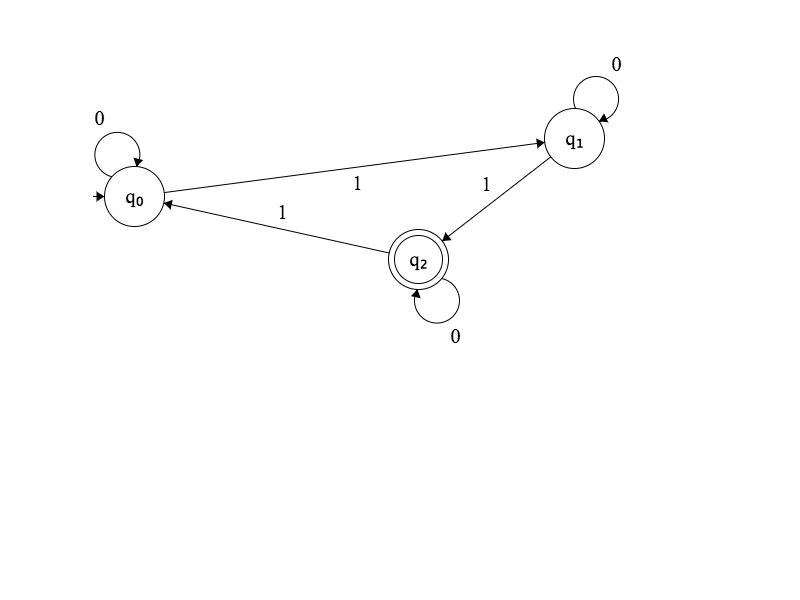
\includegraphics[width=0.8\textwidth]{img/afd.png}
  \label{fig:ejemplo}
\end{figure}

Observando la definición y aplicándola a este caso concreto podemos diferenciar:
\begin{itemize}
\item $Q=\{q_0,q_1,q_2 \}$
\item $\sum = \{0,1\}$
\item $q_0=q_0$
\item Función de transición $\delta \, t.q$:
\\
$\delta(q_0,0)=q_0 \,\,\,\,\,\,\, \delta(q_1,0)=q_1\,\,\,\,\,\,\, \delta(q_2,0)=q_2$
\\
$\delta(q_0,1)=q_1 \,\,\,\,\,\,\,  \delta(q_1,1)=q_2 \,\,\,\,\,\,\,\delta(q_2,1)=q_0$
\item $F={q_2}$
\end{itemize}
De esta forma, queda clara la correspondencia entre AFD y CMTC, sin más que comparar la definición de grafo de una CMTC con la definición de AFD.
\\\\
Podemos ver las correspondencias: $Q=E\, ,\, \sum=W$ y $| \delta |=U$ y ademas el conjunto de estados finales es el vacío, es decir, $F={\emptyset}$. 

\section{Probabilidades de transición}

Comenzamos definiendo las llamadas probabilidades de transición. Posteriormente, a partir de estas probabilidades, y restringiéndonos únicamente al caso en que la CMTC sea homogénea, construiremos la matriz de transición $P(t)$ y demostraremos sus propiedades más importantes.

Por último, partiendo de $P(t)$, generaremos y estudiaremos una nueva matriz, denominada $Q$-matriz o generador infinitesimal.

\subsection{Probabilidades de transición y matriz de transición}
\textbf{Definición: Probabilidades de transición}
\\
Dada una CMTC $\{\mathbb{X}_t \, , \, t\in [0,\infty]\}$, definimos las probabilidades de transición como:
$$p_{ij}(s,t):=P(\mathbb{X}_t=j\, | \, \mathbb{X}_s=i), \ 0\leq s < t, \ \ i,j\in S$$

A partir de este momento, supondremos que la CMTC es homogénea. Teniendo en cuenta la expresión anterior y siguiendo la definición de Cadena de Markov homogénea en tiempo continuo, citada en la sección (2.1), tenemos que la probabilidad de ir del estado $i$ al estado $j$ no depende del instante de tiempo en el que se encuentra la cadena, es decir, $p_{ij}(s,t)$ no depende de $s$ y $t$, sólo depende de la diferencia $t-s$:
$$p_{ij}(s,t)=P(\mathbb{X}_t=j\, | \, \mathbb{X}_s=i)=P(\mathbb{X}_{t-s}=j\, | \, \mathbb{X}_0=i)=p_{ij}(0,t-s)=p_{ij}(t-s)$$
Por tanto, podemos expresar las probabilidades de transición como:
$$p_{ij}(t)=P(\mathbb{X}_t=j\, | \, \mathbb{X}_0=i)=P(\mathbb{X}_{t+s}=j\, | \, \mathbb{X}_s=i)$$
siendo $t$ la diferencia entre los dos instantes de tiempo. En particular:
$$p_{ij}(0)=P(\mathbb{X}_0=j\, | \, \mathbb{X}_0=i)=\delta_{ij}:= \left\{ \begin{array}{lcc}
   	   	             1 &   si  & i=j \\
   	   	             0 &  si & i\neq j
   	   	             \end{array} \right. $$
Estamos en condiciones de construir la matriz de transición, cuyos elementos son todas las posibles probabilidades de transición:
$$P(t):=(p_{ij}(t))_{i,j\in S}$$
\textbf{Propiedades:}
\begin{enumerate}
\item Para cada $t\geq 0, \ \ p_{ij}(t)\geq 0, \ \ \forall i,j\in S$,
\item Para cada $t\geq 0, \ \ \sum\limits_{j\in S}p_{ij}(t)=1, \ \ \forall i\in S$,
\item Ecuación de \textit{Chapman-Kolmogorov}: 
$p_{ij}(s+t)=\sum\limits_{k\in S}p_{ik}(s)p_{kj}(t), \ \ \forall i,j\in S, \ \ \forall s,t\in[0,\infty)$.
\end{enumerate}

\begin{proof}
\begin{enumerate}
\item Evidente, pues $P$ es probabilidad.
\item Partiendo del hecho de que $P[\Omega]=P\left[\{\omega\in\Omega/\mathbb{X}_t(\omega)\in S\}\right]=P\left[\bigcup\limits_{j\in S}\{\omega\in\Omega/\mathbb{X}_t(\omega)=j\}\right]=P\left[\bigcup\limits_{j\in S}[\mathbb{X}_t=j]\right]=1$, tenemos:
\\\\\\
$1=P\left[\bigcup\limits_{j\in S}[\mathbb{X}_t=j]\, | \,\mathbb{X}_0=i\right]\overset{*}{=}\sum\limits_{j\in S}P\left[\mathbb{X}_t=j\, | \,\mathbb{X}_0=i\right]-\underbrace{P\left[\bigcap\limits_{j\in S}[\mathbb{X}_t=j]\, | \,\mathbb{X}_0=i \right]}_{0}=\sum\limits_{j\in S}P\left[\mathbb{X}_t=j\, | \,\mathbb{X}_0=i\right]=\sum\limits_{j\in S}p_{ij}(t)$.
\\\\

(*) $P(A_1\cup A_2\cup ... \cup A_n\, |\, B)=P(A_1\, |\,B)+P(A_2\, |\,B)+...+P(A_n\, |\,B)-P(A_1\cap A_2\cap ... \cap A_n\, |\, B)$.
\item $p_{ij}(s+t)=P\left[\mathbb{X}_{s+t}=j\, | \,\mathbb{X}_0=i\right]=P\left[\mathbb{X}_{s+t}=j, \bigcup\limits_{k\in S}[\mathbb{X}_s=k]\, | \,\mathbb{X}_0=i\right]=$

$=\sum\limits_{k\in S}P\left[\mathbb{X}_{s+t}=j,\,\mathbb{X}_s=k\, | \,\mathbb{X}_0=i\right]\overset{**}{=}$

$=\dfrac{P[\mathbb{X}_{s+t}=j,\,\mathbb{X}_s=k,\,\mathbb{X}_0=i]}{P[\mathbb{X}_0=i]}\overset{**}{=}$

$=\sum\limits_{k\in S}P\left[\mathbb{X}_{s+t}=j\, | \,\mathbb{X}_s=k, \mathbb{X}_0=i\right]P\left[\mathbb{X}_s=k\, | \,\mathbb{X}_0=i\right]\overset{CMTC}{=}$

$=\sum\limits_{k\in S}P\left[\mathbb{X}_{s+t}=j\, | \,\mathbb{X}_s=k\right]P\left[\mathbb{X}_s=k\, | \,\mathbb{X}_0=i\right]\overset{\text{Homogénea}}{=}$

$=\sum\limits_{k\in S}P\left[\mathbb{X}_t=j\, | \,\mathbb{X}_0=k\right]P\left[\mathbb{X}_s=k\, | \,\mathbb{X}_0=i\right]=\sum\limits_{k\in S}p_{kj}(t)p_{ik}(s)$.
\\\\

(**) $P(A\cap B\, | \, C)=\dfrac{P(A\cap B\cap C)}{P(C)}=P(A\, | \, B\cap C)P(B\, | \,C)$ \\
\end{enumerate}
\qed
\end{proof}

\subsection{Q-matriz o generador infinitesimal}


\textbf{Definición: Q-matriz o generador infinitesimal}
\\
Dada una CMTC $\{\mathbb{X}_t \, , \, t\in [0,\infty]\}$, con matriz de transición $P(t)$. Se define la $Q$-matriz o generador infinitesimal como:
$$Q:=\lim_{t \to 0}\dfrac{P(t)-I}{t},$$
donde $I$ es la matriz identidad del tamaño correspondiente y, por tanto, los elementos de la diagonal principal se expresan como:
$$q_{ii}=\lim_{t \to 0}\dfrac{p_{ii}(t)-1}{t}:=-q_i,$$
donde $q_i$ es la \textit{razón de escape} del estado $i$, mientras que el resto de elementos:
$$q_{ij}=\lim_{t \to 0}\dfrac{p_{ij}(t)}{t},\,\,\, i\neq j$$
donde $q_{ij}$ es llamado \textit{razón de transición} del estado $i$ al $j$.
\\\\
En lo que resta de sección, procederemos a construir esta matriz a partir de la definición de una nueva variable aleatoria. A partir de este momento, asumimos que la CMTC $\{\mathbb{X}_t \, , \, t\in [0,\infty]\}$ es continua por la derecha, es decir, si la transición de un estado $i\in S$ a un estado $j\in S$ ocurre el instante $t$, entonces se tiene que $\mathbb{X}_t=j$ y $\mathbb{X}_{t^-}=i$.

La cuestión es: ¿Dado $\mathbb{X}_0=i$, cuánto tiempo permanecerá el proceso en el estado $i$? Para responder a esta pregunta, definimos la siguiente variable aleatoria:
$$T_i\equiv \text{Tiempo que el proceso permanece en el estado} \,\, i.$$

Vamos a deducir la distribución que sigue $T_i$. Para ello será suficiente con probar que la variable $T_i$ verifica la propiedad de falta de memoria, en efecto, dados $t,s\geq 0$:
\\
$$P[T_i>s+t\, | \,T_i>s]=$$ 
$$=P[\mathbb{X}_r=i,\, para \, r\in[0,s+t]\, | \,\mathbb{X}_r=i,\, para \, r\in[0,s]]=$$
$$=P[\mathbb{X}_r=i,\, para \, r\in[s,s+t]\, | \,\mathbb{X}_r=i,\, para \, r\in[0,s]]\overset{CMTC}{=}$$
$$=P[\mathbb{X}_r=i,\, para \, r\in[s,s+t]\, | \,\mathbb{X}_s=i]\overset{\textit{Homogénea}}{=}$$
$$=P[\mathbb{X}_r=i,\, para \, r\in[0,t]\, | \,\mathbb{X}_0=i]=$$
$$=P[T_i>t].$$

Puesto que $T_i$ es una variable continua verificando la propiedad de falta de memoria, tenemos que $T_i\rightsquigarrow exp(\lambda_i)$, con $\lambda_i>0$, puesto que las únicas variables continuas que verifican esta propiedad son aquellas que siguen una distribución exponencial. Conocida la distribución de $T_i$, deducimos:
$$\mathbb{E}[T_i]=\dfrac{1}{\lambda_i},$$
y, por tanto, cuánto más grande sea el parámetro $\lambda_i$, más pequeño será el intervalo de tiempo en el que el proceso se encuentra en el estado $i$.
\\\\
Estamos preparados para construir la $Q$-matriz, $Q=(q_{ij})_{i,j\in S}$. Sea:
$$p_{ij}(T_i)=P(\mathbb{X}_{T_i}=j\, | \, \mathbb{X}_0=i), \,\, j\neq i$$
la probabilidad de transición del estado $i$ al estado $j$, definimos:
$$q_{ij}:=\lambda_i p_{ij}(T_i),\,\, i\neq j$$
la \textit{razón de transición} del estado $i$ al $j$. Para obtener los elementos de la diagonal, es decir, para el caso en que $i=j$, imponemos que la suma de los elementos de cada una de las filas de $Q$ sea $0$:
$$q_{ii}+\sum_{j\neq i}q_{ij}=0$$
$$q_{ii}=-\sum_{j\neq i}q_{ij}$$
$$q_{ii}=-\sum_{j\neq i}\lambda_i p_{ij}(T_i)$$
$$q_{ii}=-\lambda_i\underbrace{\sum_{j\neq i}p_{ij}(T_i)}_{1}$$
$$q_{ii}=-\lambda_i:=-q_i$$
y hemos obtenido $q_i$, la \textit{razón de escape} del estado $i$. Por tanto, la $Q$-matriz se puede expresar de la siguiente manera:

$$Q= \left\{ \begin{array}{lcc}
   	   	             -\sum\limits_{j\neq i}q_{ij} &   si  & i=j \\
   	   	             q_{ij} &  si & i\neq j
   	   	             \end{array} \right. $$
o equivalentemente:
$$Q= \left\{ \begin{array}{lcc}
   	   	             -\lambda_i &   si  & i=j \\
   	   	             \lambda_i p_{ij}(T_i) &  si & i\neq j
   	   	             \end{array} \right. $$

\section{Ecuación de Kolmogorov}
\section{Clasificación de los estados}
\section{Teoremas límite}
A continuación presentamos el Teorema Ergódico.
\begin{theorem}
Para una cadena de Markov irreducible se verifica:
\begin{enumerate}
\item Si todos los estados son recurrentes positivos:
$$\lim_{t\rightarrow\infty}p_{i,j}(t)=u_j>0 \, , \, \forall i,j\in S$$
Además $u=(u_j \, , \, j\in S)$ es la única distribución estacionaria de la cadena y $\displaystyle\lim_{t\rightarrow\infty}a_j (t)=u_j \, , \, \forall j\in S$. La distribución de probabilidad u es la solución del sistema $uQ=0$, siendo $Q$ la $Q$-matriz de la cadena.
\item Si todos los estados son recurrentes nulos o transitorios,
$$\lim_{t\rightarrow\infty}p_{ij}(t)=0\, , \, \forall i,j \in S\, ;\,\,\, \lim_{t\rightarrow\infty}a_j (t)=0\, , \, \forall j\in S$$
\end{enumerate}
\end{theorem}
\section{Ejemplos}
\subsection{Ejemplo 1}
\subsection{Ejemplo 2}
\end{document}}